% ********** Rozdział 2 **********
\chapter{Realizacja projektu}


\section{Opis struktury projektu}

Projekt "System Zarządzania Symulacją Samochodu" zakłada stworzenie systemu, który będzie symulować działanie samochodu w różnych warunkach drogowych, umożliwiając testowanie i analizę jego zachowania w kontrolowanych warunkach.
\begin{itemize}
    \item Klasa Samochód: Odpowiada za symulację działania samochodu, w tym kontrolę prędkości, hamowania, uwzględniając parametry techniczne i zmiany prędkości obrotowej.
    \item Klasa Silnik: Symuluje zachowanie włączenie lub wyłączenie silnika samochodu, określenie poziomu paliwa stanu oleju.
    \item Klasa Skrzynia biegów: Zarządza zmianą biegów w samochodzie i dostosowuje prędkość obrotową silnika do aktualnych warunków jazdy.
    \item Klasa Parametry: Przechowuje parametry samochodu, takie jak maksymalna prędkość, pojemność baku paliwa, średnie spalanie.
    \item Klasa Zużycie paliwa: Odpowiada za monitorowanie zużycia paliwa przez samochód w trakcie symulacji.
    \item Klasa Trasa: Symuluje trasę, po której porusza się samochód, uwzględniając różne warunki takiej jak odległość, czas podróży, średnia prędkość oraz punkt docelowy.
    \item Klasa Koszty: Zarządza obliczaniem kosztów podróży na podstawie zużycia paliwa i innych czynników.
    \item Klasa Program: Punkt wejścia do aplikacji, odpowiedzialny za uruchomienie symulacji oraz inicjalizację pozostałych komponentów.
\end{itemize}

W następnej części projektu został opracowany diagram klas, który przedstawia strukturę klas i ich relacje w ramach systemu. Diagram klas pozwala zobaczyć, jak poszczególne klasy są ze sobą powiązane, jakie są ich właściwości i metody oraz w jaki sposób komunikują się między sobą.

\begin{figure}[!ht]
	\centering
		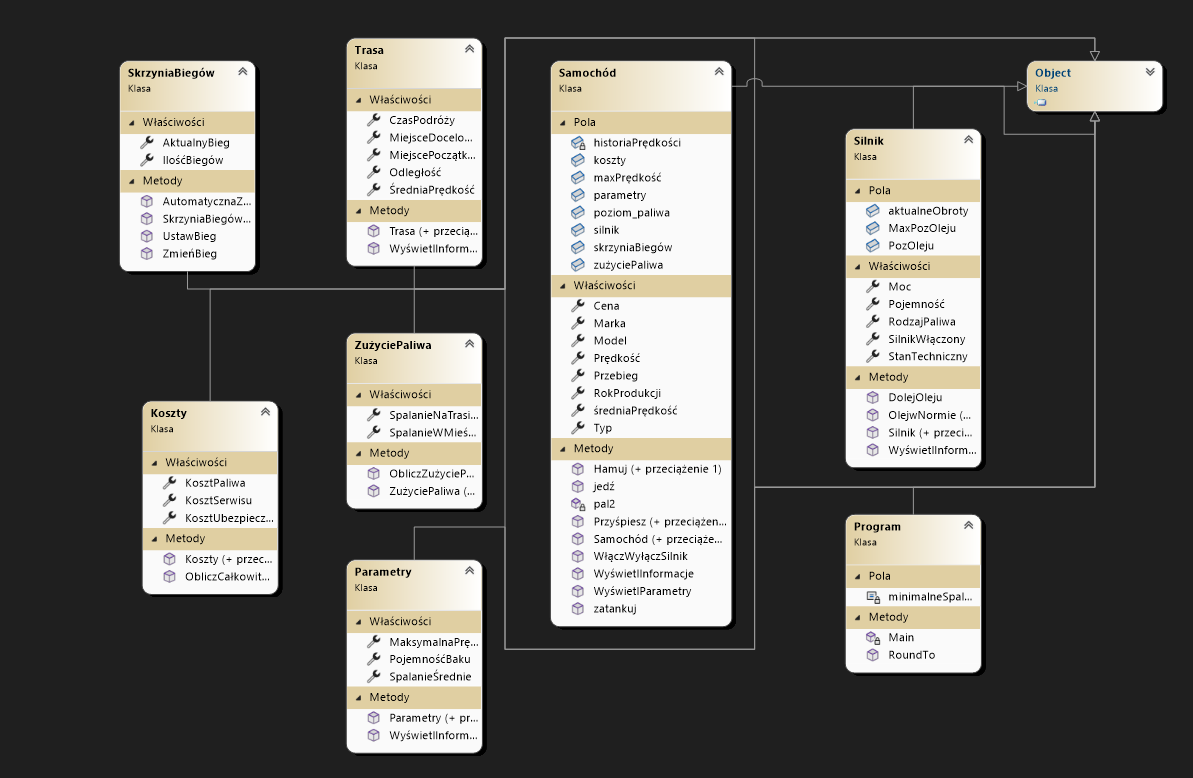
\includegraphics[width=16cm]{Diagram klas.png}
	\caption{\footnotesize Diagram klas}
	\label{fig:plotend}
\end{figure}
\newpage
\section{Opis techniczny projektu}

Projekt "System Zarządzania Symulacją Samochodu" ma na celu stworzenie kompleksowego systemu do symulacji oraz analizy zachowania pojazdu. System ten umożliwi użytkownikom interaktywne sterowanie symulowanym samochodem, monitorowanie kluczowych parametrów oraz przeprowadzanie analiz efektywności spalania, kosztów eksploatacji i innych istotnych wskaźników.
\begin{itemize}
\item .NET Framework: .NET Framework to fundamentalna platforma programistyczna, umożliwiająca rozwój różnorodnych aplikacji w języku C\# oraz innych obsługiwanych językach. Zapewnia szeroki zakres bibliotek i narzędzi, które ułatwiają tworzenie aplikacji desktopowych, webowych, serwerowych i innych. Dzięki swojej wszechstronności, .NET Framework umożliwia szybkie i efektywne rozwijanie oprogramowania.
\item Visual Studio: Visual Studio to kompleksowe środowisko programistyczne firmy Microsoft, które oferuje narzędzia do tworzenia, testowania, debugowania i zarządzania projektami. Dzięki zaawansowanym funkcjom, Visual Studio znacząco zwiększa produktywność i ułatwia rozwój aplikacji.
\item GitHub: GitHub to platforma hostingowa oparta na systemie kontroli wersji Git, która umożliwia przechowywanie kodu źródłowego, śledzenie zmian oraz współpracę zespołową nad projektem. 

Minimalne wymagania systemowe:
\begin{itemize}
    \item \textbf{System operacyjny:} Windows 10, macOS, Linux 
    \item \textbf{Procesor:} ARM64 lub x64; Zalecany czterordzeniowy lub lepszy.
    \item \textbf{Pamięć RAM:} Zalecane 4 procesory wirtualne i 16 GB pamięci RAM
    \item \textbf{Miejsce na dysku twardym:} minimalnie 850 MB
    \item \textbf{.NET:} .NET Framework lub .NET Core
\end{itemize}
\end{itemize}
\section{Zarządzanie danymi }
\begin{figure}[!ht]
	\centering
		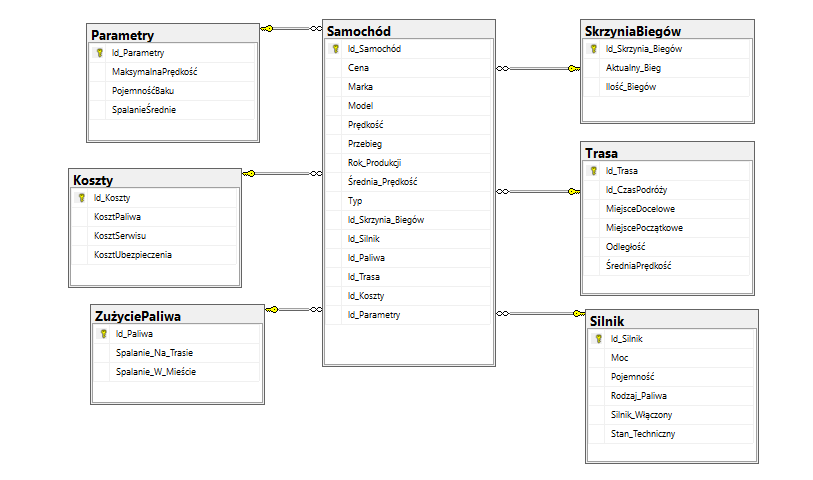
\includegraphics[width=14cm]{bazy danych.png}
	\caption{\footnotesize Schemat bazy danych}
	\label{fig:plotend}
\end{figure}
\begin{itemize}
    \item Samochód: Tabela Samochód pełni kluczową rolę jako główna tabela, łącząc relacje z innymi tabelami w systemie. Służy do przechowywania danych o samochodzie oraz zawiera klucze obce, które odnoszą się do innych istotnych aspektów pojazdu. Klucze obce umożliwiają powiązanie informacji o samochodzie z różnymi aspektami, takimi jak informacje o silniku, zużyciu paliwa, skrzyni biegów, trasy podróży, koszty eksploatacji oraz parametry techniczne. 
    \item Silnik: Tabela Silnik jest istotna dla systemu zarządzania pojazdu, ponieważ przechowuje kluczowe informacje o silniku samochodowym, co umożliwia monitorowanie ich parametrów technicznych oraz planowanie konserwacji i napraw.
    \item SkrzyniaBiegów: Tabela SkrzyniaBiegów przechowuje kluczowe informacje o skrzyni biegów w samochodzie. Te dane mogą być używane do monitorowania aktualnego biegu oraz analizy charakterystyki jazdy pojazdu.
    \item ZużyciePaliwa: Tabela ZużyciePaliwa umożliwia śledzenie zużycia paliwa przez samochód w różnych warunkach, takich jak jazda w terenie miejskim i na trasie. Informacje są istotne dla monitorowania wydajności samochodu pod względem zużycia paliwa.
    \item Trasa: Tabela Trasa umożliwia śledzenie informacji o poszczególnych trasach podróży samochodowych, dane dotyczące miejsc początkowych i docelowych, odległości pokonanej trasy oraz średniej prędkości podróżowania.
    \item Parametry: Tabela Parametry zawiera istotne informacje dotyczące parametrów technicznych samochodów, takich jak maksymalna prędkość, pojemność baku oraz średnie spalanie paliwa. 
    \item Koszty: Tabela Koszty umożliwia śledzenie kosztów związanych z eksploatacją samochodu.
\end{itemize}
% ********** Koniec rozdziału **********
